\documentclass[tikz,border=0pt]{standalone}
\usepackage{fontspec,xeCJK,unicode-math}
\setmainfont[IgnoreFontspecFile,Path=../../../字体/]{NewCM10-Book.otf}
\setCJKmainfont[Path=../../../字体/]{STSong.ttf}
\setmathfont[IgnoreFontspecFile,Path=../../../字体/]{NewCMMath-Book.otf}
\usetikzlibrary{arrows.meta}
\begin{document}
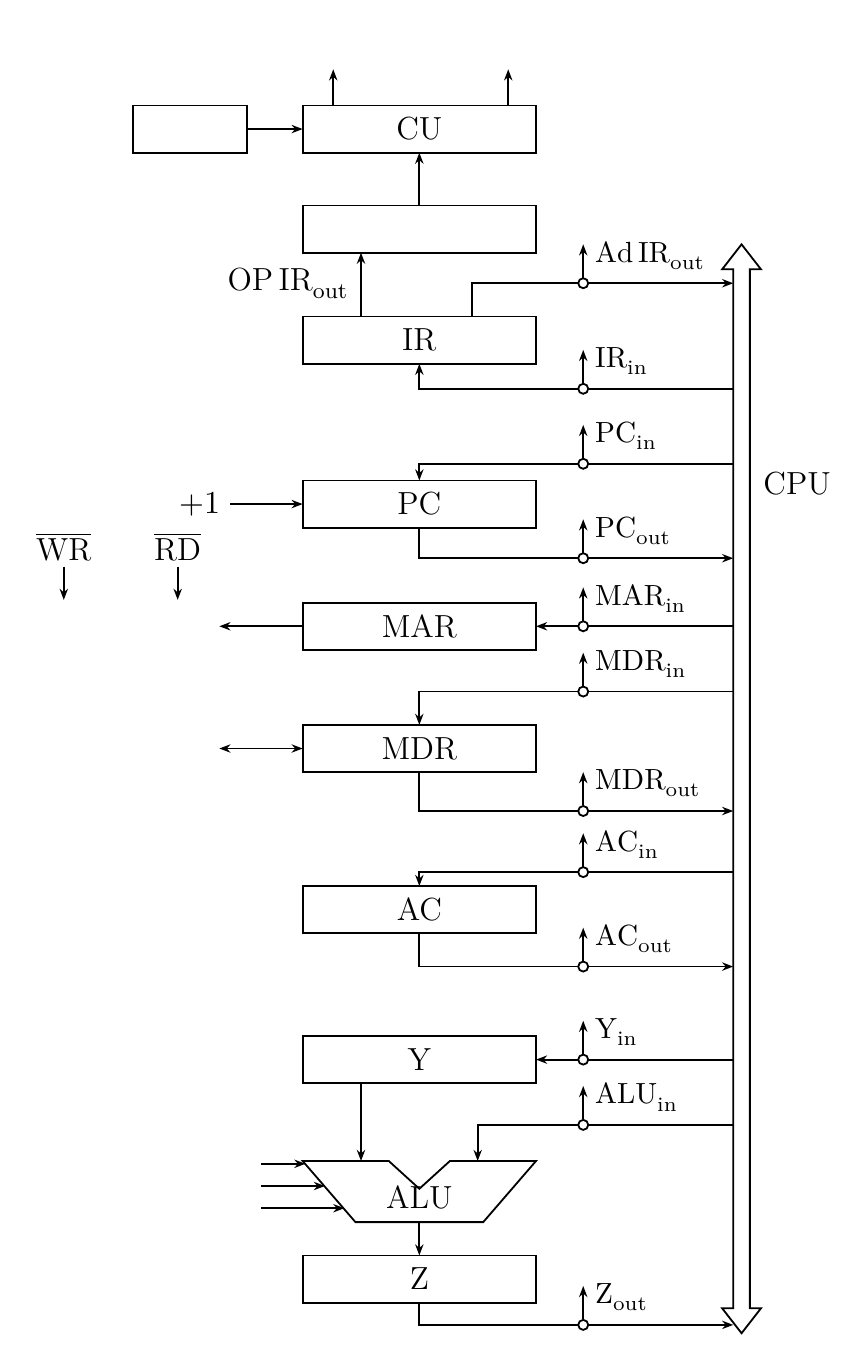
\begin{tikzpicture}[x=1bp,y=-1bp,line width=.65bp,>={Stealth[length=4bp,width=3bp]},font=\fontsize{11.5bp}{13bp}\selectfont]
\path[use as bounding box] (0,0) rectangle (290,471);
\newcommand{\reg}[2]{\draw (99,#1) rectangle ++(84,17);\node at (141,{#1+8.5}) {#2};}
\newcommand{\gate}[2]{\draw[fill=white] (200,#1) circle (1.8);\draw[->] (200,{#1-2})--(200,{#1-14});\node[anchor=west,inner sep=1bp,font=\fontsize{10.5bp}{12bp}\selectfont] at (203,{#1-10}) {#2};}
\draw (257,78)--(250,87)--(254,87)--(254,461)--(250,461)--(257,470)--(264,461)--(260,461)--(260,87)--(264,87)--cycle;
% 控制器及指令通路。
\draw (38,28) rectangle (79,45);
\node at (58.5,36.5) {时钟};
\reg{28}{CU}
\draw[->] (79,36.5)--(99,36.5);
\draw[->] (110,28)--(110,15);
\draw[->] (173,28)--(173,15);
\node[anchor=north] at (141,0) {控制信号};
\reg{64}{指令译码器}
\draw[->] (141,64)--(141,45);
\reg{104}{IR}
\draw[->] (120,104)--(120,81);
\node[anchor=east,inner sep=1bp] at (117,92) {$\mathrm{OP\,IR}_{\mathrm{out}}$};
\draw[->] (160,104)--(160,92)--(254,92);
\gate{92}{$\mathrm{Ad\,IR}_{\mathrm{out}}$}
\draw[->] (254,130)--(141,130)--(141,121);
\gate{130}{$\mathrm{IR}_{\mathrm{in}}$}
% 程序计数器与存储器接口。
\reg{163}{PC}
\draw[->] (254,157)--(141,157)--(141,163);
\gate{157}{$\mathrm{PC}_{\mathrm{in}}$}
\draw[->] (141,180)--(141,191)--(254,191);
\gate{191}{$\mathrm{PC}_{\mathrm{out}}$}
\draw[->] (73,171.5)--(99,171.5);
\node[anchor=east] at (73,171.5) {$+1$};
\reg{207}{MAR}
\draw[->] (254,215.5)--(183,215.5);
\gate{215.5}{$\mathrm{MAR}_{\mathrm{in}}$}
\draw[->] (99,215.5)--(69,215.5);
\reg{251}{MDR}
\draw[->] (254,239)--(141,239)--(141,251);
\gate{239}{$\mathrm{MDR}_{\mathrm{in}}$}
\draw[->] (141,268)--(141,282)--(254,282);
\gate{282}{$\mathrm{MDR}_{\mathrm{out}}$}
\draw[<->] (69,259.5)--(99,259.5);
\node[font=\fontsize{15bp}{17bp}\selectfont] at (37,236) {存储器};
\node at (13,187) {$\overline{\mathrm{WR}}$};
\node at (54,187) {$\overline{\mathrm{RD}}$};
\draw[->] (13,194)--(13,206);
\draw[->] (54,194)--(54,206);
% 运算数据通路。
\reg{309}{AC}
\draw[->] (254,304)--(141,304)--(141,309);
\gate{304}{$\mathrm{AC}_{\mathrm{in}}$}
\draw[->] (141,326)--(141,338)--(254,338);
\gate{338}{$\mathrm{AC}_{\mathrm{out}}$}
\reg{363}{Y}
\draw[->] (254,371.5)--(183,371.5);
\gate{371.5}{$\mathrm{Y}_{\mathrm{in}}$}
\draw (99,408)--(130,408)--(141,418)--(152,408)--(183,408)--(164,430)--(118,430)--cycle;
\node at (141,421) {ALU};
\draw[->] (120,380)--(120,408);
\draw[->] (254,395)--(162,395)--(162,408);
\gate{395}{$\mathrm{ALU}_{\mathrm{in}}$}
\node[anchor=east] at (80,414) {运算操作号};
\foreach \yy/\xx in {409/100,417/107,425/114}{\draw[->] (84,\yy)--(\xx,\yy);}
\reg{442}{Z}
\draw[->] (141,430)--(141,442);
\draw[->] (141,459)--(141,467)--(254,467);
\gate{467}{$\mathrm{Z}_{\mathrm{out}}$}
% 双向内部总线。

\node[align=center,font=\fontsize{11.5bp}{13bp}\selectfont] at (277,190) {CPU\\内\\部\\总\\线};
\end{tikzpicture}
\end{document}
